\documentclass[tikz,border=6pt]{standalone}
\usepackage{tikz}
\usetikzlibrary{angles,quotes,calc}
\definecolor{bg}{HTML}{171D2B}
\definecolor{acc}{HTML}{F7B538}
\begin{document}
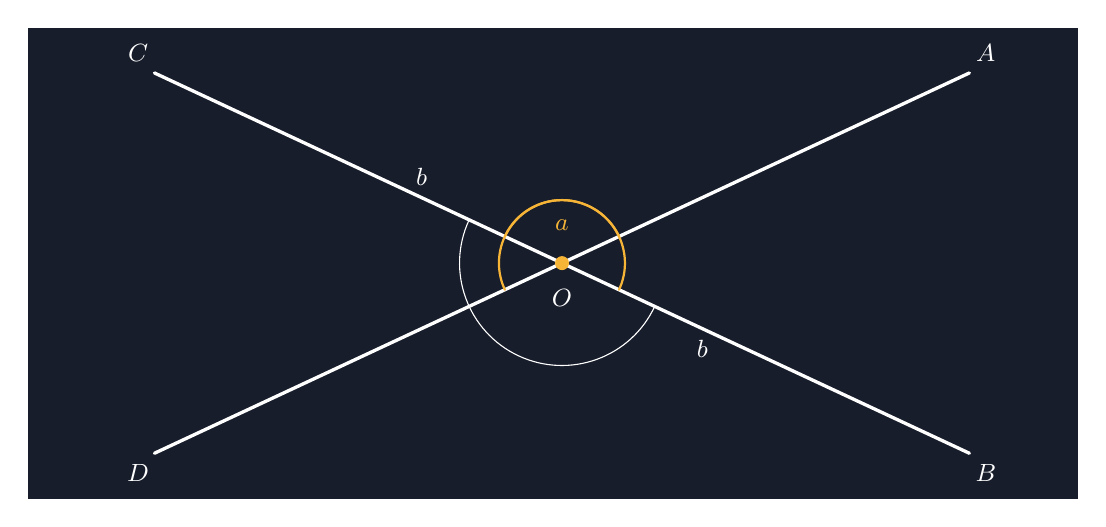
\begin{tikzpicture}[scale=1.15, line cap=round]
  \fill[bg] (-1.2,-2.6) rectangle (10.4,2.6);
  % dua garis berpotongan di O
  \draw[white, very thick] (0.2,-2.1) -- (9.2,2.1);
  \draw[white, very thick] (0.2,2.1) -- (9.2,-2.1);
  \coordinate (A) at (9.2,2.1);
  \coordinate (O) at (4.7,0);
  \coordinate (B) at (9.2,-2.1);
  \coordinate (C) at (0.2,2.1);
  \coordinate (D) at (0.2,-2.1);
  % titik potong
  \fill[acc] (O) circle (2.2pt);
  \node[white, font=\small] at ($(O)+(0,-0.38)$) {$O$};
  % label titik ujung
  \node[white, font=\small] at ($(A)+(0.18,0.22)$) {$A$};
  \node[white, font=\small] at ($(B)+(0.18,-0.22)$) {$B$};
  \node[white, font=\small] at ($(C)+(-0.18,0.22)$) {$C$};
  \node[white, font=\small] at ($(D)+(-0.18,-0.22)$) {$D$};
  % sudut a dan bertolak belakangnya
  \pic[draw=acc, thick, angle radius=8mm, "$a$"{acc, font=\small, fill=bg, inner sep=1pt}] {angle=A--O--C};
  \pic[draw=acc, thick, angle radius=8mm, "$a$"{acc, font=\small, fill=bg, inner sep=1pt}] {angle=B--O--D};
  % sudut berpelurus (b)
  \pic[draw=white!60, thin, angle radius=13mm] {angle=C--O--B};
  \node[white!70, font=\small] at ($(O)+(1.55,-0.95)$) {$b$};
  \node[white!70, font=\small] at ($(O)+(-1.55,0.95)$) {$b$};
\end{tikzpicture}
\end{document}
